\chapter{APPROSSIMAZIONE DI FUNZIONI}
\section{Esercizio 14}

\textit{\textbf{Descrizione:} Scrivere un programma che implementi efficientemente il calcolo del polinomio interpolante su un insieme di ascisse distinte.}\newline

\noindent\emph{Soluzione: }\newline

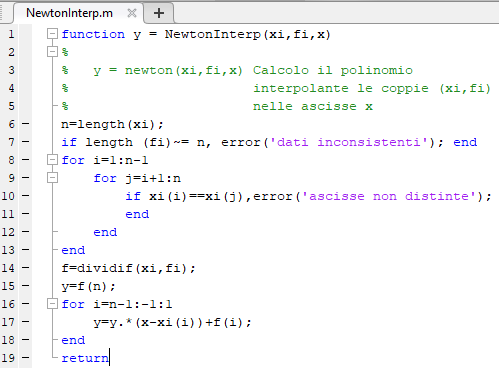
\includegraphics[width=1.3\linewidth]{img/NewtonInter.png}
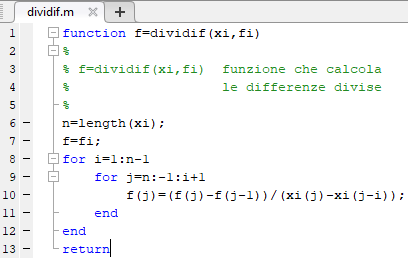
\includegraphics[width=1.3\linewidth]{img/dividif.png}\newpage